% !TEX program = XeLaTeX
% !TEX encoding = UTF-8

\documentclass[a4paper]{article}

\usepackage[UTF8]{ctex}
\usepackage{graphicx}
\usepackage{soul, color, xcolor}
\usepackage[margin=1.25in]{geometry}
\usepackage{amsfonts, amsmath, amsthm, bm, amssymb}
\usepackage{float}
\usepackage{diagbox}
\usepackage{multirow}
\usepackage{hyperref}
\usepackage{listings}
\usepackage{tcolorbox}

\lstset{basicstyle=\tiny}

\setlength{\parindent}{0pt}

\numberwithin{equation}{section}

\theoremstyle{definition}
\newtheorem*{solution}{Solution}
\newtheorem*{prove}{Proof}

\def \transposed {\mathsf{T}}
\def \hermitian {\mathsf{H}}
\def \Real {\mathbb{R}}
\def \betaBold {\bm{\beta}}
\def \LambdaBold {\bm{\Lambda}}
\def \MuBold {\bm{\Mu}}
\def \muBold {\bm{\mu}}
\def \Sw {\mathbf{S}_{\mathrm{w}}}
\def \Sb {\mathbf{S}_{\mathrm{b}}}
\def \St {\mathbf{S}_{\mathrm{t}}}
\def \A {\mathbf{A}}
\def \B {\mathbf{B}}
\def \C {\mathbf{C}}
\def \O {\mathbf{O}}
\def \Q {\mathbf{Q}}
\def \I {\mathbf{I}}
\def \S {\mathbf{S}}
\def \M {\mathbf{M}}
\def \W {\mathbf{W}}
\def \X {\mathbf{X}}
\def \u {\bm{u}}
\def \v {\bm{v}}
\def \w {\bm{w}}
\def \wh {\hat{\bm{w}}}
\def \ws {\bm{w}^\star}
\def \y {\bm{y}}
\def \x {\bm{x}}
\def \xh {\hat{\bm{x}}}

% \let\oldnorm\norm
% \let\norm\undefined
\newcommand\abs[1]{\left| #1 \right|}
\newcommand\norm[1]{\left\| #1 \right\|}
\newcommand\inner[2]{\left\langle #1, #2 \right\rangle}
\newcommand\sbr[1]{\left( #1 \right)}
\newcommand\mbr[1]{\left[ #1 \right]}
\newcommand\lbr[1]{\left\{#1 \right\}}
\newcommand\tr[1]{\mathrm{tr}\sbr{#1}}
\newcommand\rank[1]{\mathrm{rank}\sbr{#1}}
\newcommand\indicator[1]{\mathbb{I}\sbr{#1}}

\begin{document}

\title{机器学习导论 习题二}
\author{221300079, 王俊童, \href{mailto:221300079@smail.nju.edu.cn}{221300079@smail.nju.edu.cn}}
\maketitle

\section*{作业注意事项}

\begin{tcolorbox}
	\begin{enumerate}
		\item[1.] 作业所需的LaTeX及Python环境配置要求请参考: \href{https://www.lamda.nju.edu.cn/ML2024Spring/supplementary/environment.pdf}{[Link]};
		\item[2.] 请在LaTeX模板中第一页填写个人的学号、姓名、邮箱;
		\item[3.] 本次作业需提交的文件与对应的命名方式为:
		      \begin{enumerate}
			      \item [(a)] 作答后的LaTeX代码 --- \texttt{HW2.tex};
			      \item [(b)] 由(a)编译得到的PDF文件 --- \texttt{HW2.pdf};
			      \item [(c)] 编程题代码 --- \texttt{main.py};
		      \end{enumerate}
		      请将以上文件{\color{red}\textbf{打包为 ``\texttt{学号\hspace{0em}\_\hspace{0em}姓名.zip}''}}~(例如 ``\texttt{221300001\_\hspace{0em}张三.zip}'') 后提交;
		\item[3.] 若多次提交作业, 则在命名 ``\texttt{.zip}'' 文件时加上版本号, 例如 ``\texttt{221300001\_\hspace{0em}张三\hspace{0em}\_v1.zip}'' (批改时以版本号最高, 提交时间最新的文件为准);
		\item[4.] 本次作业提交截止时间为~{\color{red}\textbf{{4}月{19}日{23:59:59}}}. 未按照要求提交作业, 提交作业格式不正确, {\color{red}\textbf{作业命名不规范}}, 将会被扣除部分作业分数; 除特殊原因 (如因病缓交, 需出示医院假条) 逾期未交作业, 本次作业记 0 分; {\color{red}\textbf{如发现抄袭, 抄袭和被抄袭双方成绩全部取消}};
		\item[5.] 学习过程中, 允许参考 ChatGPT 等生成式语言模型的生成结果, 但必须在可信的信息源处核实信息的真实性; {\color{red}\textbf{不允许直接使用模型的生成结果作为作业的回答内容}}, 否则将视为作业非本人完成并取消成绩;
		\item[6.] 证明题请给出关键证明步骤, 计算题请列出算式及中间结果, 否则不予计分; 撰写数学表达式请遵循符号约定.
		\item[7.] 本次作业提交地址为 \href{https://box.nju.edu.cn/u/d/a84222be492048779a27/}{[Link]}, 请大家预留时间提前上交, 以防在临近截止日期时, 因网络等原因无法按时提交作业.
	\end{enumerate}
\end{tcolorbox}

\newpage

\section*{符号约定}

\textbf{[线性代数变量符号]} 本次作业的部分题目涉及矩阵形式的数学推导, 请注意符号规范.

提示: 可以在导言区通过 \texttt{\textbackslash{def}}, \texttt{\textbackslash{newcommand}} 等命令自定义常用符号以简化编写, 例如 \texttt{\textbackslash{Real}}, \texttt{\textbackslash{norm}} 等.

\begin{itemize}
	\setlength\itemsep{0em}
	\item 矩阵请使用\textbf{粗体正体字母}, 例如 $\A, \X, \O$ (零矩阵);
	\item 向量请使用\textbf{粗体斜体字母}, 例如 $\u, \v, \w, \x, \y, \bm{0}$ (零向量);
	\item 标量(以及离散变量)请使用\textbf{斜体小写字母}, 例如 $a, b, c, \lambda, \mu, \sigma$;
	\item 操作符或者函数名请使用\textbf{正体有衬线体字母}, 例如 $\min, \max, \mathrm{Ent}, \mathrm{MI}$;
	\item 转置矩阵 (Transposed Matrix) 以及埃尔米特矩阵 (Hermitian Matrix) 的\textbf{角标}请使用\textbf{正体无衬线体字母}, 例如 $\A^\transposed, \A^\hermitian$.
	% 注意: 请\textbf{不要}使用斜体字母 $T, H$, $\A^T, \A^H$ 将被视作矩阵之幂; 请\textbf{不要}使用 \texttt{\textbackslash{top}}, \texttt{\textbackslash{bot}}, $\top, \bot$ 常用于几何学, 逻辑学和抽象代数.
\end{itemize}

\textbf{[奇异值分解与特征值分解]} 由于 $\Real^n \times \Real^m$ 上存在全序关系, 我们可以约定, 存在一种奇异值分解过程, 在此奇异值分解过程的意义下, 任何矩阵的奇异值分解是唯一的, 进而\textbf{任何(半)正定矩阵的特征值分解也是唯一的}. 如果没有符号冲突, 可以不加说明的使用以下记号:

\begin{itemize}
	\setlength\itemsep{0em}
	\item 矩阵 $\A \in \Real^{n \times m}$ 的\textbf{奇异值分解}是 $\A = \sum_{i=1}^{\min\{m,n\}} \sigma_i \u_i \v_i^\transposed$, $\sigma_i \geqslant \sigma_{i+1}$;
	\item \textbf{(半)正定} 矩阵 $\A \in \Real^{n \times n}$ 的\textbf{特征值分解}是 $\A = \sum_{i=1}^{n} \lambda_i \v_i \v_i^\transposed$, $\lambda_i \geqslant \lambda_{i+1}$;
	\item 另记 $\sigma_{\max}(\A) = \sigma_1(\A), \lambda_{\max}(\A) = \lambda_1(\A)$ 是矩阵 $\A$ 最大的奇异值.
\end{itemize}

\textbf{[决策树]} 为简化表述, 我们引入指示函数 $\indicator{e}$: 若事件 $e$ 发生, 则 $\indicator{e} = 1$, 否则 $\indicator{e} = 0$. 对于\textbf{表格数据}, 我们约定:

\begin{itemize}
	\setlength\itemsep{0em}
	\item 每个样例 $\x$ 都具有 $d$ 个属性 $\{1, \cdots, d\}$;
	\item 第 $j$ 个属性有 $n_j$ 种可能的取值, 记作 $\x^j \in \{v^j_1, \cdots, v^j_{n_j}\}$;
	\item 对于多分类问题, 样例的标签可以记作 $\x^\ell$, 共有 $N$ 种可能取值, 即 $\x^\ell \in \{1, \cdots, N\}$.
\end{itemize}

例如: 对于数据集 $D = \{\x_1, \cdots, \x_m\}$, 事件 $\x^j = v^j_k$ 的频率值可以记作 $\hat{p}(\x^j = v^j_k) = \frac{1}{m} \sum_{i=1}^{m} \indicator{\x_i^j = v^j_k}$; 再如, 对于 ``西瓜数据集2.0'' (详见教材表4.1), 记号示范如下:

\begin{itemize}
	\setlength\itemsep{0em}
	\item $d = 6$;
	\item $\x^1 \in \{v^1_1=\text{乌黑}, v^1_2=\text{青绿}, v^1_3=\text{浅白}\}$, 即第1个属性色泽, $n_1 = 3$;
	\item $\x^2 \in \{v^2_1=\text{蜡缩}, v^2_2=\text{稍蜷}, v^2_3=\text{硬挺}\}$, 即第2个属性根蒂, $n_2 = 3$;
	\item $\x^3 \in \{v^3_1=\text{清脆}, v^3_2=\text{浊响}, v^3_3=\text{沉闷}\}$, 即第3个属性敲声, $n_3 = 3$;
	\item $\x^4 \in \{v^4_1=\text{清晰}, v^4_2=\text{稍糊}, v^4_3=\text{模糊}\}$, 即第4个属性纹理, $n_4 = 3$;
	\item $\x^5 \in \{v^5_1=\text{凹陷}, v^5_2=\text{稍凹}, v^5_3=\text{平坦}\}$, 即第5个属性脐部, $n_5 = 3$;
	\item $\x^6 \in \{v^6_1=\text{软粘}, v^6_2=\text{硬滑}\}$, 即第6个属性触感, $n_6 = 2$.
\end{itemize}

\newpage

\section{[20pts] 岭回归}

在本题中, 我们假设\textbf{所有凸优化问题均有解}.

回顾教材第三章第二节, 多元线性回归相当于求解如下的无约束优化问题 \eqref{lr}. 其中, 对于 $\v \in \Real^d$, 定义 $\norm{\v}_2^2 = \v^\transposed \v$.
\begin{equation}
	\min_{\wh} \quad\norm{\X\wh - \y}_2^2
	\label{lr}
\end{equation}
在多元线性回归中增加约束项, 即成为\textbf{岭回归 (Rigde Regression}), 即求解有约束优化问题 \eqref{ridge-rho}, 其中 $\rho > 0$ 是待确定的超参数.
\begin{equation}
	\begin{aligned}
		\min_{\wh} \quad  & \norm{\X\wh - \y}_2^2           \\
		\text{s.t.} \quad & \norm{\wh}_2^2 \leqslant \rho^2 \\
	\end{aligned}
	\label{ridge-rho}
\end{equation}
岭回归也可以写成无约束优化问题 \eqref{ridge-lambda}. 其中, $\lambda > 0$ 是待确定的超参数.
\begin{equation}
	\begin{aligned}
		\min_{\wh} \quad\norm{\X\wh - \y}_2^2 + \lambda \norm{\wh}_2^2
	\end{aligned}
	\label{ridge-lambda}
\end{equation}

\begin{itemize}
	\item[(1)] \textbf{[5pts]} 相比于多元线性回归, 岭回归引入了额外的\textbf{归纳偏好 (Inductive Bias)}. 回顾教材第一章第四节, 请简要回答: 岭回归引入了怎样的归纳偏好? 这样的归纳偏好有怎样的作用? \\
	      提示: 回顾\textbf{过拟合 (Overfitting)、``奥卡姆剃刀'' (Occam's Razor) 原则}等知识点; 结合特殊情形回答, 例如矩阵 $\X$ 不满秩、数据中存在异常值等.
	\item[(2)] \textbf{[5pts]} 请证明岭回归的两种形式 \eqref{ridge-rho} 和 \eqref{ridge-lambda} 等价. \\
	      提示:考虑 \textbf{KKT条件 (Karush-Kuhn-Tucker Conditions)}.
	\item[(3)] \textbf{[5pts]} 对于无约束优化形式 \eqref{ridge-lambda}, 假设 $\lambda$ 已经确定, 此时岭回归的解记作 $\ws$, 请推导出 $\ws$ 的表达式.
	\item[(4)] \textbf{[5pts]} \textbf{在 (3) 的基础上}, 请推导出 $\lambda$ 的下界 (关于 $\rho$ 的函数), 并据此回答: $\rho$ 减小时, 若希望保持 \eqref{ridge-rho} 和 \eqref{ridge-lambda} 的解一致, 需要怎样调整 $\lambda$? \\
	      提示: 你可能需要引入 $\sigma_{\max}(\X)$.
\end{itemize}

\begin{solution}
	\textbf{(1)}.岭回归引入了一个额外的L2正则化项,通过这个L2正则化项来引入器归纳偏好。L2正则化项的处理还是很常见的,可以使得模型更加稳定,可以处理一些异常情况。这个归纳偏好的作用有:\\
	\textbf{1}.正则化项限制了模型的大小,这样相当于一个惩罚加入模型中,从而限制了模型的复杂度,有利于阻碍过拟合。\\
	\textbf{2}.岭回归减少了参数值的大小,使得模型更加的简单化了,符合了”奥卡姆剃刀“原则,尽量的在保证数据拥有足够解释的情况下使得模型简洁。\\
	\textbf{3}.对于不满秩矩阵,传统的多元线性回归事找不到唯一最小二乘解的,岭回归加入正则化项使得其可以计算出稳定解\\
	\textbf{4}.如果数据有异常的值需要处理,岭回归可以减少异常值对于模型的影响,可以通过缩小参数值来限制模型对于数据点的敏感度。\\
	\textbf{(2)}.这两个一定是等价的,对于1.2:根据拉格朗日乘子法,可得\\
	\[
		L(\hat{w}, \lambda) = || \mathbf{X}\hat{w} - \mathbf{y} ||_2^2 + \lambda ( || \hat{w} ||_2^2 - \rho^2)
	\]
	对于这个式子,我们有kkt条件得到:\\
	1.求导为0\[
		2\mathbf{X}^T (\mathbf{X}\hat{w} - \mathbf{y}) + 2\lambda \hat{w} = 0
	\]
	2.原始条件:$||\hat{w}||_2^2 \leq \rho^2$\\
	3.对偶条件:$\lambda>0$\\
	4.互补松弛条件:$\lambda(||\hat{w}||_2^2 - \rho^2) = 0$、、
	所以当以上条件成立的时候,原问题的1.2就可以以1.3的形式来表达出岭回归:
	\[
		\min_{\wh} \quad\norm{\X\wh - \y}_2^2 + \lambda \norm{\wh}_2^2
	\]
	\textbf{(3)}.若$\lambda$已经确定了,我们可以通过解这个目标函数来得到解答:
	\[
		f(\hat{w}) = || \mathbf{X}\hat{w} - \mathbf{y} ||_2^2 + \lambda || \hat{w} ||_2^2
	\]
	计算梯度:
	\[
		\nabla f(\hat{w}) = 2\mathbf{X}^T ( \mathbf{X}\hat{w} - \mathbf{y}) + 2\lambda \hat{w}
	\]
	等于0,可得到:
	\[
		2\mathbf{X}^T ( \mathbf{X}\hat{w} - \mathbf{y}) + 2\lambda \hat{w} = 0
	\]
	\[	
		( \mathbf{X}^T \mathbf{X} + \lambda \mathbf{I}) \hat{w} = \mathbf{X}^T \mathbf{y}
	\]
	\[
		\hat{w} = ( \mathbf{X}^T\mathbf{X} + \lambda \mathbf{I})^{-1} \mathbf{X}^T\mathbf{y}
	\]

	\textbf{(4)}.首先我们已经得到了:
	\[
		\hat{w} = ( \mathbf{X}^T\mathbf{X} + \lambda \mathbf{I})^{-1} \mathbf{X}^T\mathbf{y}
	\]
	我们引入这个函数$\sigma_{max} (\mathbf{X})$,本身这个值可以作为一个上界,通过约束条件,我们可以得到:
	\[
		(( \mathbf{X}^T \mathbf{X} + \lambda \mathbf{I})^{-1} \mathbf{X}^T y)^T((\mathbf{X}^T \mathbf{X} + \lambda \mathbf{I})^{-1} \mathbf{X}^T y) - \rho^2 \leq 0 	
	\]
	根据矩阵的奇异值分解,矩阵X的最大奇异值是 $\sigma_{max}(X)$,所以对应于无约束情况下$\lambda$的下界,我们可以得到:
	\[
		(\mathbf{X}^T \mathbf{X} + \lambda \mathbf{I})^{-1} \rightarrow \sigma(\mathbf{X})^2 + \lambda \geq 0	
	\]
	对于$\mathbf{X}^T \mathbf{X} + \lambda \mathbf{I}^{-1}$做奇异值分解,得到$\mathbf{V} \Sigma \mathbf{V}^T$,其中$\Sigma \leq ((\sigma_{max}(X)^2 + \lambda)^{-1} \mathbf{I}) \mathbf{X^T} y  \leq \rho^2 $,所以带回
	到原式,我们可以得到:
	\[
		\lambda \geq \frac{||\mathbf{X^T} y||}{\rho} - \sigma_{max}(\mathbf{X})^2
	\]	

	在这个式子里面,里面的部分是正定的,所以$\sigma(X)$
	所以对于这种情况下,若$\rho$减少,$\lambda$应当增加。
\end{solution}

\newpage

\section{[20pts] 决策树的构建流程}

\begin{tcolorbox}
	\textbf{[注意事项]} 本题可使用 PowerPoint\textsuperscript{\textregistered}, Visio\textsuperscript{\textregistered} 等软件软件绘制决策树, 导出为图片或 PDF 插入到作业文档中; 亦允许手绘决策树, 但是请确保文字与线条的工整. 如果插入照片, 请确保照片内容清晰可读, 否则将扣除部分分数.
\end{tcolorbox}

考虑如下的表格数据集: 在诊断疾病 RD 时, 通常采用 UW-OCT, OCT-PD, US 三种检测手段, 其中 1 代表阳性, 0 代表阴性. 假设总共收集了 16 位病人的检测结果, 其中 8 条用于训练, 如表格 \ref{dt-train} 所示, 8 条用于验证, 如表格 \ref{dt-valid} 所示.

\begin{table}[ht]
	\centering
	\setlength{\abovecaptionskip}{0pt}
	\setlength{\belowcaptionskip}{5pt}
	\caption{训练集 $D_{\mathrm{train}}$}
	\label{dt-train}
	\begin{tabular}{cccc|c}
		\hline
		编号 & UW-OCT & OCT-PD & US & RD \\
		\hline
		1  & 1      & 1      & 0  & 1  \\
		2  & 1      & 1      & 1  & 1  \\
		3  & 0      & 1      & 1  & 1  \\
		4  & 0      & 1      & 1  & 1  \\
		5  & 0      & 0      & 1  & 0  \\
		6  & 1      & 0      & 0  & 0  \\
		7  & 1      & 0      & 1  & 0  \\
		8  & 0      & 1      & 0  & 0  \\
		\hline
	\end{tabular}
\end{table}

\begin{table}[ht]
	\centering
	\setlength{\abovecaptionskip}{0pt}
	\setlength{\belowcaptionskip}{5pt}
	\caption{验证集 $D_{\mathrm{valid}}$}
	\label{dt-valid}
	\begin{tabular}{cccc|c}
		\hline
		编号 & UW-OCT & OCT-PD & US & RD \\
		\hline
		9  & 1      & 1      & 1  & 1  \\
		10 & 0      & 1      & 1  & 1  \\
		11 & 0      & 1      & 0  & 0  \\
		12 & 1      & 0      & 1  & 0  \\
		13 & 0      & 1      & 1  & 1  \\
		14 & 1      & 1      & 0  & 0  \\
		15 & 1      & 0      & 0  & 0  \\
		16 & 0      & 0      & 0  & 0  \\
		\hline
	\end{tabular}
\end{table}

\begin{enumerate}
	\item[(1)] \textbf{[10pts]} 回顾教材第四章第一, 二节, 请使用基尼指数作为划分准则, 通过训练集中的数据训练决策树. 在 \texttt{HW2.pdf} 中展示\textbf{最终得到的决策树}, 并给出\textbf{每个节点划分时的计算和比较过程}.
	\item[(2)] \textbf{[5pts]} 回顾教材第四章第三节, 在(1)的基础上, 请判断每个节点是否需要预剪枝. 在 \texttt{HW2.pdf} 中展示\textbf{预剪枝后的决策树}, 并给出\textbf{每个节点预剪枝时的计算和比较过程}.
	\item[(3)] \textbf{[5pts]} 对一个学习任务来说, 给定属性集, 其中有些属性可能很关键, 很有用, 称为 ``相关特征'', 另一些属性则可能用处不大, 称为 ``无关特征''. 请简要回答如下问题:
	      \begin{itemize}
		      \item[(a)] 比较 (1,2) 的结果, 指出当前训练集和验证集划分下的无关特征, 并说明理由.
		      \item[(b)] 如果不给出数据集, 只给出决策树和剪枝后的决策树, 应该怎样挑选无关特征?
		      \item[(c)] 如果不给出数据集, 也不给出剪枝后的决策树, 只给出未剪枝的决策树, 还能挑选无关特征吗? 请简要给出理由.
	      \end{itemize}
\end{enumerate}

\begin{solution}
	(1)对于整个数据集而言:$gini\_index(D)= 1 - \frac{1}{4} - \frac{1}{4} = \frac{1}{2} $\\
    第一次划分:\\
    $gini\_index(D,UW.OCT = 1) =gini\_index(D,UW.OCT = 0) =\frac{4}{8}(1- (\frac{1}{2})^2 - (\frac{1}{2})^2) + \frac{4}{8}(1 - (\frac{1}{2})^2 - (\frac{1}{2})^2) = \frac{1}{2}$\\
    $gini\_index(D,OCT.PD = 1) =gini\_index(D,OCT.PD = 0) =\frac{5}{8}(1- (\frac{4}{5})^2 - (\frac{1}{5})^2  + \frac{3}{8}(1 - 1)) = \frac{1}{5}$\\
    $gini\_index(D,US = 1) =gini\_index(D,US = 0) = \frac{2}{5}(1 - 1) + \frac{3}{5}(1 - (\frac{2}{3})^2 - (\frac{1}{3})^2) = \frac{4}{15}$\\
    根据决策树判定规则,我们可以得到第一次划分的选择应该是OCT.PD.$\frac{1}{5} < \frac{4}{15} < \frac{1}{2}$.\\
    第二次划分:\\
    $gini\_index(D,UW.OCT = 1) = gini\_index(D,UW.OCT = 0) =\frac{2}{5}(1-1) + \frac{3}{5}(1 - (\frac{2}{3})^2 - (\frac{1}{3})^2) = \frac{4}{15}$\\
    $gini\_index(D,US = 1) = gini\_index(D,US = 0) = \frac{2}{5}(1 - (\frac{1}{2})^2 - (\frac{1}{2})^2) = \frac{1}{5}$\\
    根据决策树判定规则,我们可以得到第二次划分的选择应该是US.$\frac{1}{5} < \frac{4}{15}$.\\
    第三次划分也就显而易见了,把剩下的属性划分了就行,于是我们可以得到如下的决策树:\\
    \begin{figure}[H]
		\centering
		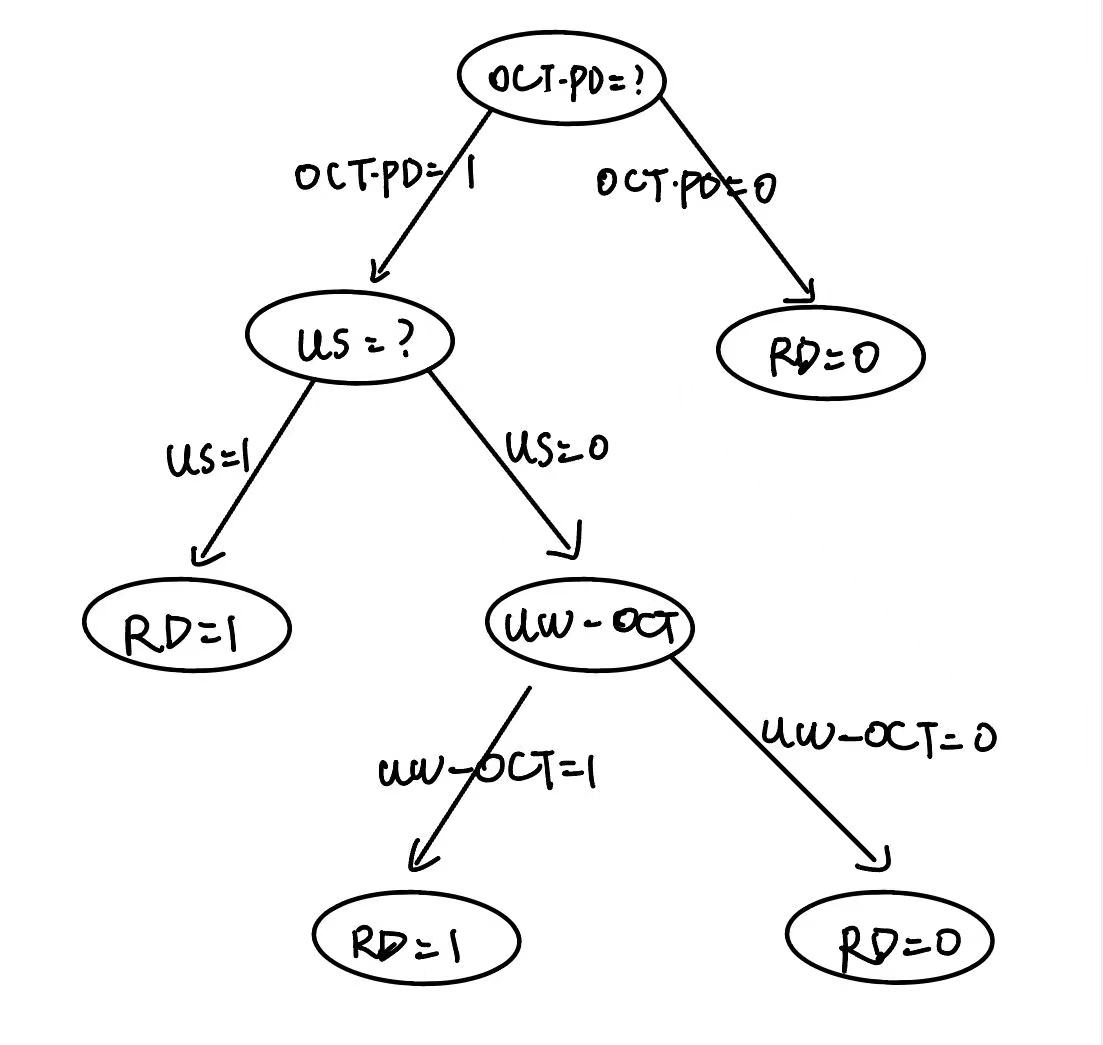
\includegraphics[width=0.7\textwidth]{DT.png}
		\caption{DT}
		\label{fig:roc0}
	\end{figure}
    (2).根据预剪枝的定义,我们可以得到如下预剪枝结果:蓝色的表示测试集样例划分\\
    但是由于我们的UW-OCT这个节点我们在训练集上是一个好一个坏,我们并不知道预测成为何种情况,所以会有两个划分模式:\\
    \textbf{在正常的划分里面,这种划分通常是随机的(4.10日课后询问周志华老师得知),因为期望是一样的}\\
    划分1:UW-OCT是好的。\\
    \begin{figure}[H]
		\centering
		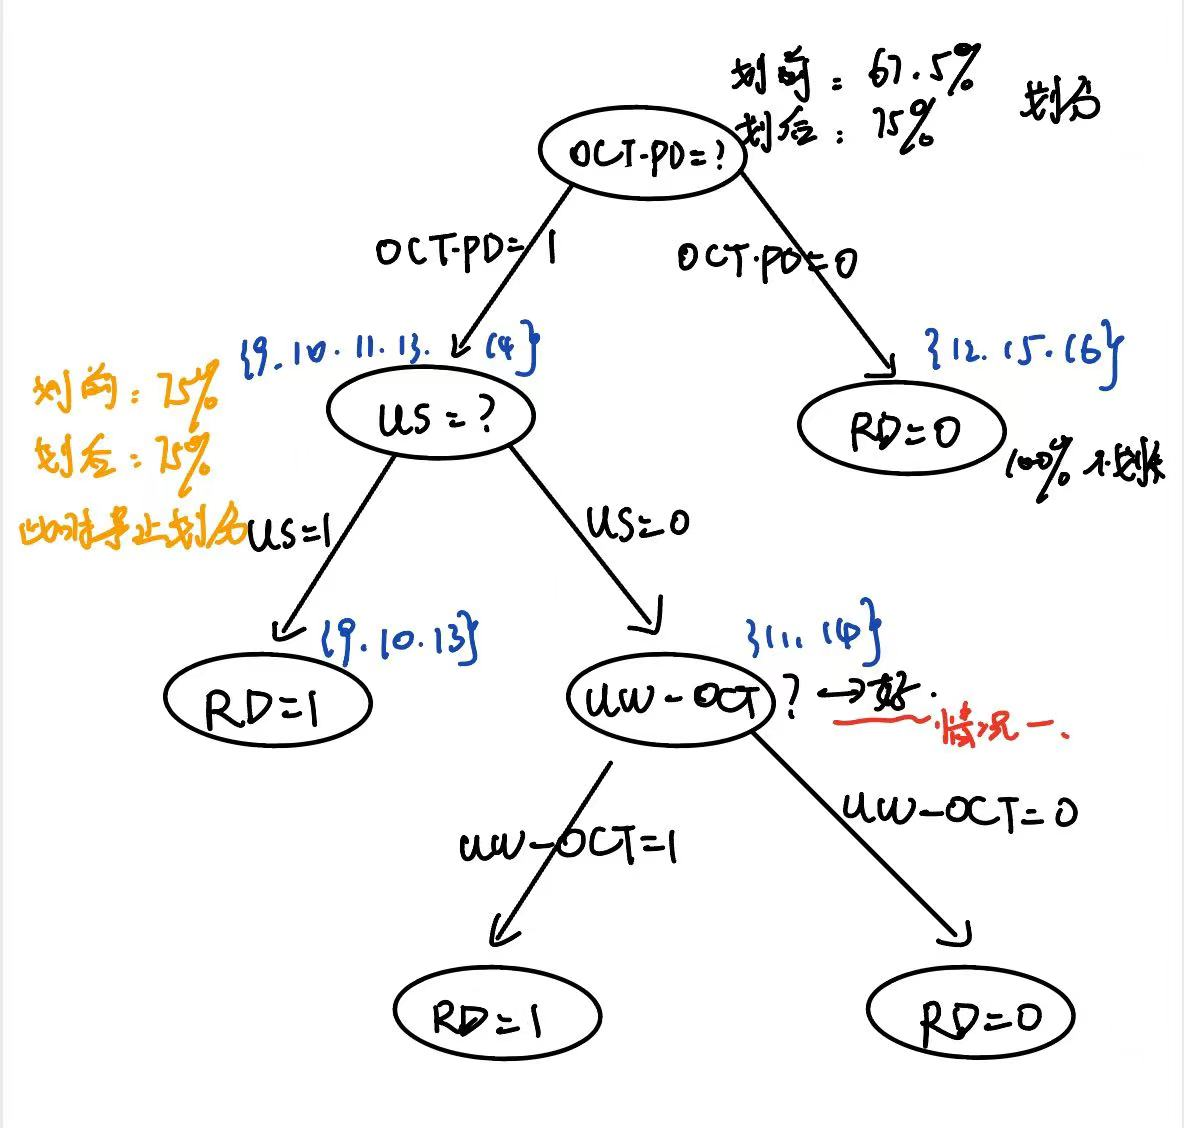
\includegraphics[width=0.7\textwidth]{Pre1.png}
		\caption{Pre1}
		\label{fig:roc1}
	\end{figure}
    划分2:UW-OCT是坏的。\\
    \begin{figure}[H]
		\centering
		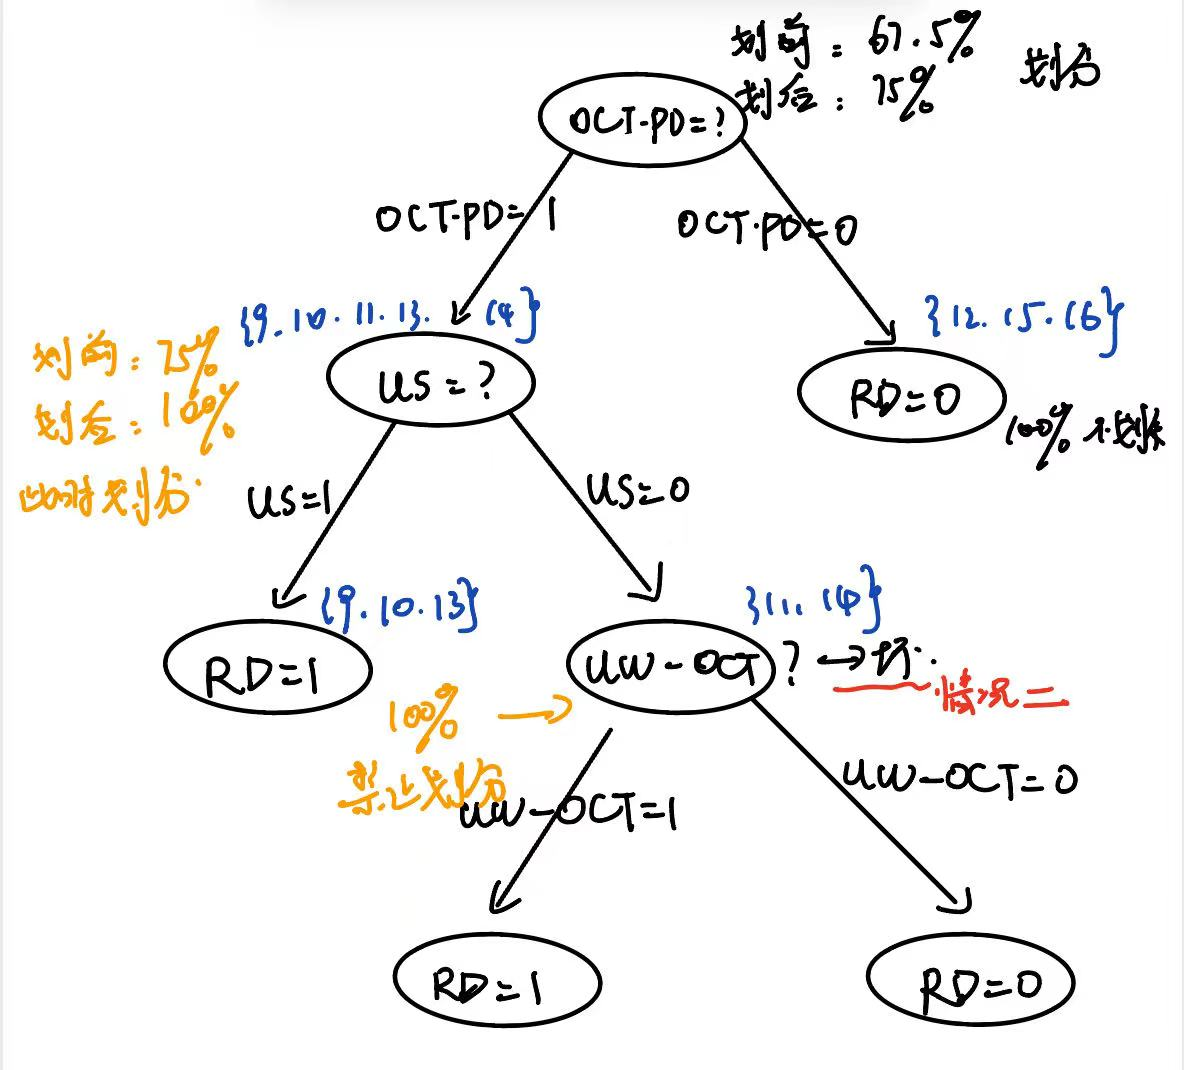
\includegraphics[width=0.7\textwidth]{Pre2.png}
		\caption{Pre2}
		\label{fig:roc2}
	\end{figure}
\end{solution}
    (3).\\
    (a).无关特征应该是UW-OCT这一个特征:理由如下\\
    对于UW-OCT而言,无论是情况1还是情况2,我们的划分在测试集上都表明我们的树对于UW-OCT的划分需求是不需要的。所以这个划分对于我们最后的影响是可有可无的,用处不大,属于无关特征。\\
    (b).若只给出决策树和剪枝后的决策树,被剪掉的决策树中的部分就是无关特征,因为剪枝操作告诉了我们这一部分是无关紧要的,所以挑选无关特征就是被剪掉的部分。\\
    (c).其实是可行的,但是我觉得如果只有决策树的话我们的判断会受到一定的限制。\\
    首先可以明确的是未剪枝的决策树里面或多或少存在一些无关信息,比如噪音,那么对于这些东西,应当是可以观察到哪些分支对于特征分类的贡献是较小的,可以分析一下特征的重要性和深度,一般来说过于深的决策树会过拟合,所以应该是有办法只在知道决策树的情况下完成这个选择的。
\newpage

\section{[15pts] 决策树的划分准则}

\begin{enumerate}
	\item[(1)] \textbf{[5pts]} 回顾教材第四章第一节, 请结合\textbf{决策树基本算法中递归返回的条件}, 简要回答: 如果要求 ``只要训练集不含冲突数据(即特征向量完全相同但标记不同), 就必须获得与训练集一致 (即训练误差为 $0$) 的决策树'', 那么纯度函数需要满足怎样的要求?
	\item[(2)] \textbf{[5pts]} 回顾教材第四章第二节, 信息增益可以重写成互信息 (Mutual Information)
	      $$\mathrm{MI}(E,F) = \sum_{e \in E} \sum_{f \in F} p(e,f) \log \frac{p(e,f)}{p(e)p(f)},$$
	      其中 $E,F$ 都是事件的集合. 请给出此时 $E,F$ 的定义, 列出必要的推导步骤, 并使用 $\mathrm{MI}(E,F)$, $\mathrm{Ent}(E)$, $\mathrm{Ent}(F)$ 等符号表示增益率.
	\item[(3)] \textbf{[5pts]} 考虑归一化互信息 (Normalized Mutual Information) 的一种定义
	      $$\mathrm{NMI}(E,F) = \frac{\mathrm{MI}(E,F)}{\sbr{\mathrm{MI}(E,E) + \mathrm{MI}(F,F)} / 2} = \frac{2 \cdot \mathrm{MI}(E,F)}{\mathrm{Ent}(E) + \mathrm{Ent}(F)}.$$
	      \textbf{在 (3) 的基础上}, 如果使用归一化互信息作为划分准测, 与使用增益率作为划分准测产生的决策树相同吗? 请给出证明或举出反例. \\
	      提示: 已知数学性质 $0 \leqslant \mathrm{MI}(E,F) \leqslant \min\{\mathrm{Ent}(E), \mathrm{Ent}(F)\}$.
\end{enumerate}

\begin{solution}
	(1).\\
    首先,在不断划分的过程中,纯度显然是越来越高的,叶子节点纯度应为100\%, 而当一个分支下样本是一半一半的时候,纯度是最低的,为50\%,在决策树的递归返回的条件中:\\
    条件1:完全属于同一类别,这时候纯度就是100\%,纯度函数应该是最大的这个时候.\\
    条件2:选不出来,包含样本集合为空,这时候纯度就在最大和最小之间了.\\
    条件3:选不出来,所有属性取值一样,这时候选择最大的类别作为集合点归属,这时候纯度也在最大和最小之间,有可能达到最小。\\
    (2).\\
    E代表特征的不同取值,F代表类别标签的不同取值(目标特征)。根据信息论的观点,互信息$I(X,Y)$应该是知道了X之后Y的不确定性减少了多少,所以在决策树里面我们用E和F这样写应该也是对的。\\
    下面是公式推导MI:首先是边缘分布和联合分布\\
    \[
        H(E) = -\sum_{e \in E}p(e)log p(e), \quad H(F) = -\sum_{f \in E}p(f)log p(f)
    \]
    \[
        H(E, F) = - \sum_{e in E} \sum_{f in F} p(e,f) log p(e,f)
    \]
    然后我们可以得到:\\
    \[
        \mathrm{MI}(E,F) = H(E) +H(F) - H(E,F)  
    \]
    所以我们化简之后可以得到:\\
    $$\mathrm{MI}(E,F) = \sum_{e \in E} \sum_{f \in F} p(e,f) \log \frac{p(e,f)}{p(e)p(f)},$$
    根据增益率的定义:\\
    $$gain\_ratio = \frac{\mathrm{MI}}{valids Information}$$
    所以可以得到:\\
    $$gain\_ratio = \frac{\mathrm{MI}(E,F)}{\mathrm{Ent}(E)}$$
    (3).\\
    根据定义可以得到;\\
    $$\mathrm{NMI}(E,F) = \frac{\mathrm{MI}(E,F)}{\sbr{\mathrm{MI}(E,E) + \mathrm{MI}(F,F)} / 2} < \frac{2 \cdot \min\{\mathrm{Ent}(E), \mathrm{Ent}(F)\} }{\mathrm{Ent}(E) + \mathrm{Ent}(F)}.$$
    显然划分是不大一样的,两者运用的计算方法都不大一样,归一化互信息考量的是两个信息之间的依赖性,而增益率是在属性固有值的程度上进行考量的。举一个例子:
    \begin{table}[ht]
        \centering
        \setlength{\abovecaptionskip}{0pt}
        \setlength{\belowcaptionskip}{5pt}
        \caption{example}
        \label{example}
        \begin{tabular}{ccc|c}
            \hline
            编号 & feature1 & feature2  & RD \\
            \hline
            1 & 1      & 1      & 1  \\
            2 & 1      & 0      & 0  \\
            3 & 0      & 1      & 0  \\
            4 & 0      & 0      & 0  \\
            \hline
        \end{tabular}
    \end{table}
    在这个例子里面,如果按照信息增益作为划分,feature1和feature2的信息增益都是0.311。而且两者的归一化互信息也一样。
    所以对于这个例子,决策树的划分很显然可能是不一样的。所以这种情况下有多个划分情况,可能产生不同.或者说,如果两个feature完全独立,是可能导致不同划分结果的。
    (我也不大会)
\end{solution}
\newpage

\section{[20(+5)pts] 线性判别分析 }

回顾教材第三章第四节, LDA (Linear Discriminant Analysis) 有两个优化目标: 最小化类内散度 $\w^\transposed \Sw \w$ 与最大化类间散度 $\w^\transposed \Sb \w$, \textbf{目的是使得同类样例的投影点尽可能接近, 异类样例的投影点尽可能远离}. 在LDA之外,课堂上还介绍了PCA (Principal Components Analysis, 主成分分析). 事实上, PCA可以写成类似LDA的形式, 但PCA只有一个目标, 即最大化全局散度: $\max_{\w} \w^\transposed \St \w$.

\begin{enumerate}
	\item[(1)] \textbf{[5pts]} 教材图 3.3 中, ``\textbf{+}'', ``\textbf{-}'' 代表数据点, 任务需要把二维数据降维到一维, 直线 $y = \w^\transposed \x$ 代表LDA的投影方向. 请画出图 \ref{textbook_fig_3_3} 数据集上\textbf{PCA的大致投影方向} (可以使用蓝色直线), 并在 \texttt{HW2.pdf} 中展示.
	      \begin{figure}[htbp]
		      \centering
		      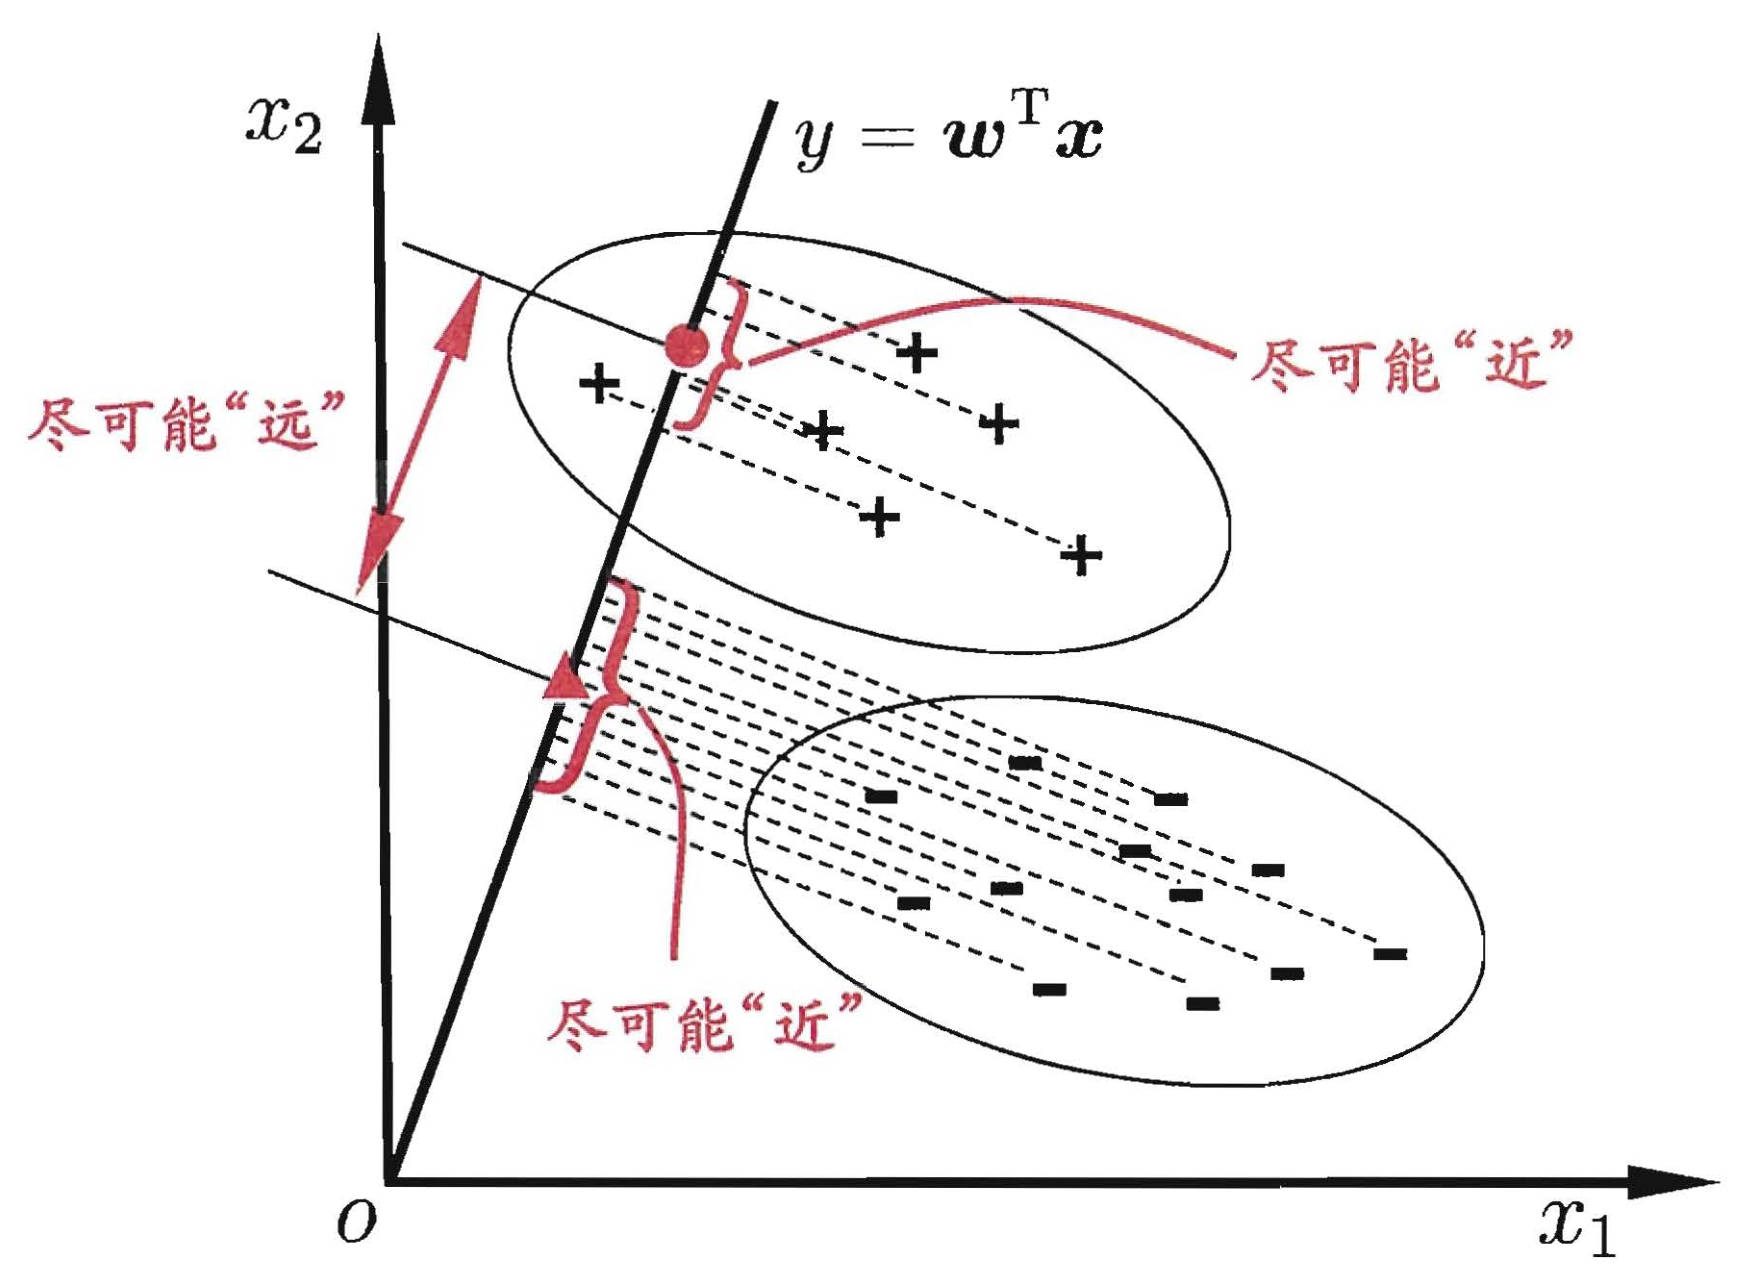
\includegraphics[width=0.5\linewidth]{textbook-fig3.3.jpg}
		      \caption{教材图 3.3}
		      \label{textbook_fig_3_3}
	      \end{figure}
	\item[(2)] \textbf{[5pts]} 请参考题干中的介绍与 (1) 中的现象, 简要回答:
	      \begin{itemize}
		      \item [(a)] 对照题干中LDA的优化目的, PCA的优化目的是什么?
		      \item [(b)] PCA相较于LDA有什么显著的不同点?
	      \end{itemize}
	\item[(3)] \textbf{[5pts]} \textit{下面, 我们先回顾教材第三章第四节中多分类 LDA 优化问题的矩阵形式. 考虑总类内散度是各个类别散度之和, 其矩阵形式为:
		      $\Sw = \sum_{i=1}^{N} {\Sw}_i.$
		      对于第 $i$ 个类别的类内散度矩阵定义如下:
		      ${\Sw}_i = \sum_{\x \in X_i} (\x - \muBold_i) (\x - \muBold_i)^\transposed.$
		      类似的, 总类间散度是各个类别中心相对于全局中心的散度之和, 其矩阵形式为:
		      $\Sb = \sum_{i=1}^{N} {\Sb}_i.$
		      对于第 $i$ 个类别的中心相对于全局中心的散度矩阵定义如下:
		      ${\Sb}_i = m_i (\muBold_i - \muBold) (\muBold_i - \muBold)^\transposed.$}\\
	      LDA事实上是在最小化\textbf{平均}类内散度和最大化\textbf{平均}类间散度, 其矩阵形式如 \eqref{lda-eigen} 所示. 其中, $d'$ 是降维后的维度, 严格小于数据维度 $d$.
	      \begin{equation}
		      \begin{aligned}
			      \max_{\W} \quad     & J(\W) = \frac{\tr{\W^\transposed \Sb \W}}{\tr{\W^\transposed \Sw \W}} = \frac{\tr{\W^\transposed \sbr{\sum_{i=1}^{N} {\Sb}_i} \W}}{\tr{\W^\transposed \sbr{\sum_{i=1}^{N} {\Sw}_i} \W}} = \frac{\frac{1}{N} \sum_{i=1}^{N} \tr{\W^\transposed {\Sb}_i \W}}{\frac{1}{N} \sum_{i=1}^{N} \tr{\W^\transposed {\Sw}_i \W}} \\
			      \mathrm{s.t.} \quad & \W^\transposed \W = \I_{d'}
		      \end{aligned}
		      \label{lda-eigen}
	      \end{equation}

	      \textbf{根据教材中的介绍, \eqref{lda-eigen} 可通过广义特征值分解进行求解.} 然而, 在某些现实场景下, 我们应用LDA的目的是提高分类准确率, 那么通常进一步希望\textbf{每个}类别散度尽可能小, \textbf{每个}类别中心相对于全局中心的散度尽可能大, \textbf{而非平均散度}. 因此, 考虑LDA的一种拓展形式:
	      \begin{equation}
		      \begin{aligned}
			      \max_{\W} \quad     & \sbr{\min_{i,j} J_{i,j}(\W)} = \frac{\min_{j} \{ \tr{\W^\transposed {\Sb}_j \W} \}}{\max_{i} \{ \tr{\W^\transposed {\Sw}_i \W} \}} \\
			      \mathrm{s.t.} \quad & \W^\transposed \W = \I_{d'}
		      \end{aligned}
		      \label{lda-pairwise}
	      \end{equation}
	      \textbf{请指出拓展形式 \eqref{lda-pairwise} 无法直接沿用原有形式 \eqref{lda-eigen} 的广义特征值求解算法的原因.} \\
	      提示: 指出求解时存在变量间的循环依赖关系.
	\item[(4)] \textbf{[5pts]} \textit{在线性代数中, 对于(半)正定矩阵 $\A, \B$, 若 $\sbr{\A-\B}$ 是正定矩阵, 则通常记作 $\A \succ \B$ 或 $\B \prec \A$; 若 $\sbr{\A-\B}$ 是半正定矩阵, 则通常记作 $\A \succcurlyeq \B$ 或 $\B \preccurlyeq \A$. 在优化问题中, 凸优化问题有多项式时间复杂度的理论保证, 能够高效求解. 凸优化问题的定义是: (i) 最小化的目标函数是凸函数, 或者最大化的目标函数是凹函数, 而且 (ii) 可行域是凸集合. 可行域是所有满足约束条件的控制变量取值 (又称可行解) 构成的集合.} \\
	      拓展形式 \eqref{lda-pairwise} 不能沿用原有形式 \eqref{lda-eigen} 的求解算法, 也不是凸优化问题. 为了高效求解, 需要探索一种将其转化成凸优化问题的方法. 已知原有形式 \eqref{lda-eigen} 可以松弛成如下凸优化问题:
	      \begin{equation}
		      \begin{aligned}
			      \max_{\W,r} \quad   & r                                             \\
			      \mathrm{s.t.} \quad & r \cdot \tr{\Sw \M} - \tr{\Sb \M} \leqslant 0 \\
			      \quad               & -r \leqslant 0                                \\
			      \quad               & \O \preccurlyeq \M \preccurlyeq \I_{d'}       \\
			      \quad               & \tr{\M} = d'                                  \\
		      \end{aligned}
		      \label{lda-slack}
	      \end{equation}
	      请仿照原有形式 \eqref{lda-eigen} 的松弛形式 \eqref{lda-slack}, 给出拓展形式 \eqref{lda-pairwise} 的松弛形式, 并证明拓展形式的松弛形式是凸优化问题, 即同时满足条件 (i) 和条件 (ii).
	\item[(5)] \textbf{[5pts]} (\textit{本题为附加题, 得分计入卷面分数, 但本次作业总得分不超过 100 分}) 请证明:
	      \begin{itemize}
		      \item [(a)] 松弛形式 \eqref{lda-eigen} 和原有形式 \eqref{lda-slack} 的约束条件不等价;
		      \item [(b)] 当 $r \cdot \tr{\Sw \M} - \tr{\Sb \M} = 0$ 时, \eqref{lda-slack} 的可行域是 \eqref{lda-eigen} 可行域的凸包 (Convex Hull). 即: \eqref{lda-slack} 的可行解可以表示成 \eqref{lda-eigen} 的可行解的线性组合.
	      \end{itemize}
	      进而, \eqref{lda-slack} 的可行域是包含 \eqref{lda-eigen} 的可行域的最小凸集合, 即 \eqref{lda-slack} 对 \eqref{lda-eigen} 的放松程度是最小的, 因而能够使得凸问题 \eqref{lda-slack} 的解尽可能的接近原问题 \eqref{lda-eigen} 的解.
\end{enumerate}

\begin{solution}
	\textbf{(1)}.根据LDA和PCA的不同,大概可以得到如下的图:
	\begin{figure}[H]
		\centering
		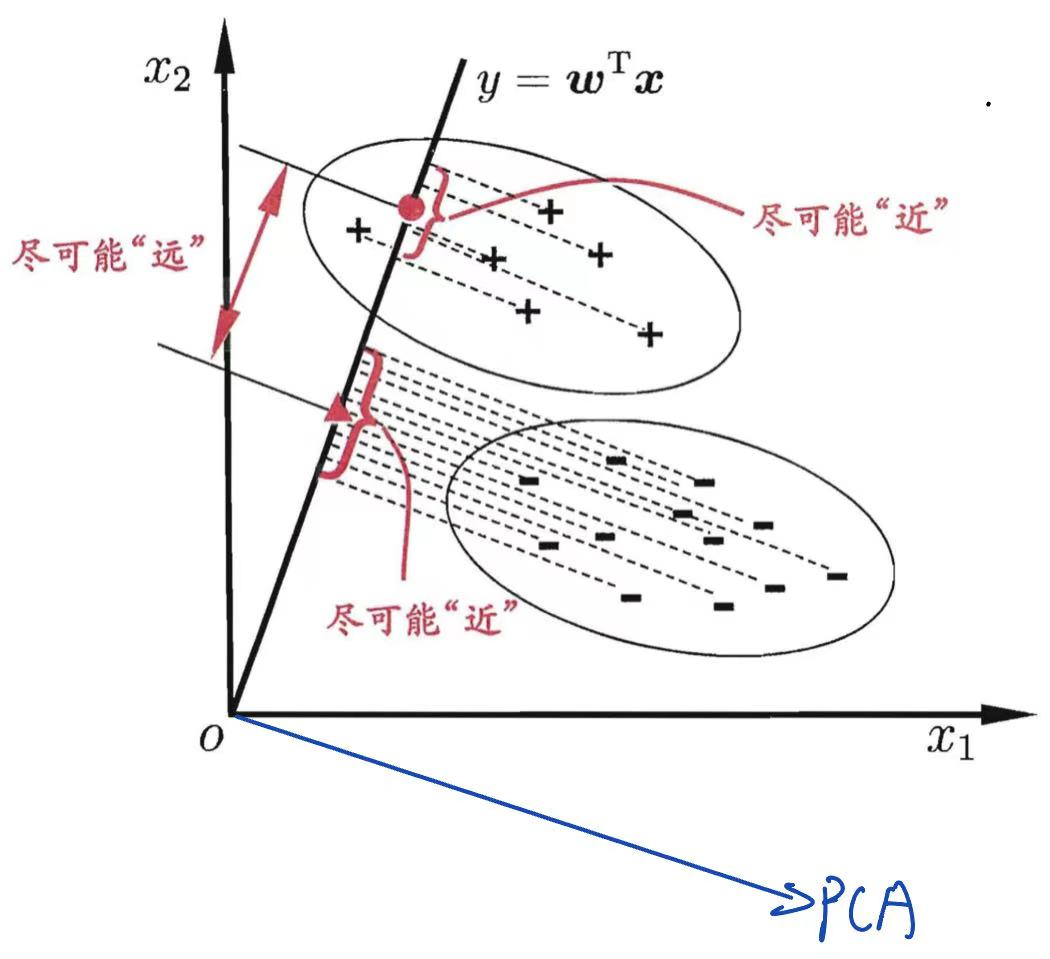
\includegraphics[width=0.7\textwidth]{1.png}
		\caption{Approximately PCA}
		\label{fig:roc1}
	\end{figure}
	\textbf{(2)}.\\
	(a).PCA跟LDA相比,其优化目的是最大化数据的方差,在把数据投影到新的坐标系进行将为之后,尽可能的最大化方差。\\
	(b).\\
	1.首先,PCA是无监督的,没有label,而LDA是一种有监督的,有label。\\
	2.其次PCA的目的是最大化方差来找数据的主要特征,而LDA是保留一种最好区分不同类别的特征。\\
	3.PCA得到的是投影方向中数据最大方差的方向,而LDA得到的投影方向是捕捉到类别间差异最大的方向。\\
	4.PCA 忽略了类别信息,只关注数据整体的结构;而 LDA 利用了类别信息,在降维同时尽可能地保留了数据不同类别之间的差异性。\\
	\textbf{(3)}.对于式子4.1,这个式子里面是在最大化类间散度并最小化类内散度的基础上进行求解的,这样是没问题的,但是延拓式子4.2指出,在最小化
	类内散度并最大化类间散度的最大最小范式下去求解,这样涉及了对于每个类别内部散度和每个类别之间的最大最小化,这样就导致了变量间的循环依赖关系,因为
	计算类内散度和类间散度时需要用到 W ,而选择 W 又依赖于类内散度和类间散度的计算结果,这就死循环了,这样就不好,所以无法用广义特征值求解算法。\\
	\textbf{(4)}.根据式子4.1的结果,我们可以得到4.3的结果如下:
	\begin{equation}
		\begin{aligned}
		& \min_{i,j} \quad -r_{ij}\\                                            
		& \mathrm{s.t.} \quad  r_{ij} \cdot \tr{\mathbf{S_{wi}} \M_{ij}} - \tr{\mathbf{S_{bj}} \M_{ij}} \leqslant 0 \\
		& -r_{ij} \leqslant 0    \\
		& \O \preccurlyeq \M_{ij} \preccurlyeq \I_{d'}  \\
		& \tr{\M_{ij}} = d'  \\
		\end{aligned}
	\label{equation}
	\end{equation}
	接下来我们证明i1和i2.对于拓展问题而言\\
	对于i1,最小化的目标函数是凸函数,对于出现的min$r_{ij}$来说是一个目标函数凸函数,然后对于tr来说也是正交的,满足性质\\
	对于i2,可行域是个凸集合,tr是正交的,不等式约束也是线性约束,矩阵约束也是半正定的,线性等式就不用说了,综上分析约束条件都是凸集合,所以可行域是凸集合。\\
	\textbf{(5)}.\\
	(a).对于4.1,只有正交矩阵约束:
	\[
		\mathbf{M^T}\mathbf{M} = \mathbf{I_{d'}}	
	\]
	对于问题4.3,我们化简之后有三个约束条件:
	\begin{equation}
		\begin{aligned}                                        
			\mathrm{s.t.} \quad & r \leq \frac{\tr{\Sb \M}}{\tr{\Sw \M}}        \\
			\quad               & \O \preccurlyeq \M \preccurlyeq \I_{d'}       \\
			\quad               & \tr{\M} = d'                                  \\
		\end{aligned}
		\label{lda1-slack}
	\end{equation}
	若要证明两者是不一样的,我们需要构造一个特殊解可以将两个约束条件区分开来。\\
	对于问题4.1,当 ( d' = 1 ),$\W$可以是任何单位向量,因为任何单位向量乘以其转置都会得到1\\
	对于问题4.3,当 ( d' = 1 ),$\M$必须是一个$1 \times 1 $的矩阵,其值在0和1之间,且迹等于1。这意味着$\M$必须是1。
	假设我们构造一个$\Sb,\Sw$满足半正定条件,我们选择$\W$为任何的一个单位向量,就满足4.1了,但是$\M$并不满足4.3的约束,因为4.3需要$\tr{\Sb},\tr{\Sw}$来共同决定.换而言之,不一定正交。\\
    (b).在(a)中也提到了,如果我们的条件是一个等式,我们其实可以得到这是一个及其特殊的情况:\\
	\[
		r = \frac{\text{tr}(\Sb \M)}{\text{tr}(\Sw \M)}    
	\]
   	而此时r要大于等于0,这个形式对于4.1而言,根据凸集合的定义,解出可得:
    \[
        \tr{\theta \M + (1-\theta) \M }= \theta\tr{\M} + (1-\theta)\tr{\M} = \tr{M} = d' 
    \]
    所以这是个凸集合,即4.5的可行解可以表示成4.1的线性组合,满足凸优化的定义,同时我们所有的$\tr{\M} = \lambda_1 + ... + \lambda_n = d'$,若满足4.1的条件,这个矩阵一定正定,所以肯定是原问题的最小凸集合。所以可以证明这是个凸包。
\end{solution}

\newpage

\section{[25pts] 编程实验: LDA 与多分类}

\begin{tcolorbox}
	\textbf{[注意事项]} 请不要修改或提交 \texttt{utils.py}; 在合理范围内, 运行时间和错误率不作为评分依据. 实现过程中只允许使用 NumPy 和 SciPy 提供的矩阵运算接口, 否则相应题目不计入分数.

	此外, 对于题 (3,4,5), 如果调用 Sci-Kit Learn 实现二分类模型, 基于二分类模型实现多分类模型, 并且画出相应图像, 可计入题 (4,5) 得分, 但不计入题 (3) 得分.

	\textbf{[符号约定]} \texttt{x} 是形状为 \texttt{(m, d)} 的矩阵, 其元素为32位浮点数; 在题 (1,3,4,5) 中, \texttt{y} 是形状为 \texttt{(m,)} 的向量, 其元素为32位整数; 在题 (2) 中, \texttt{y} 是形状为 \texttt{(m, 2)} 的向量, 其元素为32位浮点数. 其中: \texttt{m} 为样例个数, \texttt{d} 为样例维度; 标签从 \texttt{0} 开始, 例如共20类时, 标签依次是 $\{\mathtt{0}, \cdots, \mathtt{19}\}$.
\end{tcolorbox}

\begin{enumerate}
	\item[(1)] \textbf{[5pts]} 根据 \texttt{main.py} 中的框架代码, 实现LDA降维, 通过 \texttt{lda\_sanity\_check} 测试, 并在 \texttt{HW2.pdf} 中展示运行后的终端输出截图.
	\item[(2)] \textbf{[5pts]} 基于 (1) 分别把训练数据和测试数据降至两维, 并绘制在同一张散点图上, 在 \texttt{HW2.pdf} 中展示. 注意: 同类别的点应当使用同一颜色, 不同类别的数据点应当使用不同颜色.
	\item[(3)] \textbf{[5pts]} 分类任务可以被归结为一种特殊的回归任务, 可参考 \texttt{sklearn} 中的内容: \href{https://scikit-learn.org/stable/modules/linear_model.html#classification}{[Link]}. 对于二分类任务, 我们任选一类作为正类, 另一类成为负类. 对于正类样本 $\x_+$, 约定 $y_+ = 1$, 对于负类样本 $\x_-$, 约定 $y_- = -1$, 对于训练得到的分类器 $f$ 和测试样例 $\x$, 如果 $f(\x) \geqslant 0$ 预测为正类, 否则预测为负类. \\根据框架代码, 按照上述约定实现基于岭回归的二分类模型, 通过\\ \texttt{classifier\_2\_sanity\_check} 测试, 并在 \texttt{HW2.pdf} 中展示运行后的终端输出截图.
	\item[(4)] \textbf{[5pts]} 基于 (3) 中的二分类模型, 通过 OvR 策略将其拓展为多分类模型, 通过\\ \texttt{classifier\_n\_sanity\_check} 测试, 最后在 \texttt{HW2.pdf} 中展示运行后的终端输出截图.\\提示: 判断测试样例的预测结果时, 可以依照教材实现, 即若有多个分类器预测为正类或者没有分类器预测为正类, 则考虑各分类器的预测置信度 ($f(\x)$ 之值), 选择置信度最大的类别标记作为分类结果.
	\item[(5)] \textbf{[5pts]} 基于 (4) 绘制并在 \texttt{HW2.pdf} 中展示\textbf{训练错误率和测试错误率随 $\lambda$ 变化的折线图}. 注意: 图像横轴为 $\lambda$; 训练错误率和测试错误率应当使用不同颜色的曲线.
\end{enumerate}

\begin{solution}
	(1):截图如下:\\
    \begin{figure}[H]
		\centering
		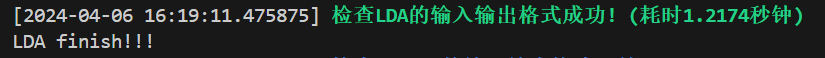
\includegraphics[width=0.7\textwidth]{LDA.png}
		\caption{LDA test}
		\label{LDA test}
	\end{figure}
    (2).得到的图如下:\\
    \begin{figure}[H]
		\centering
		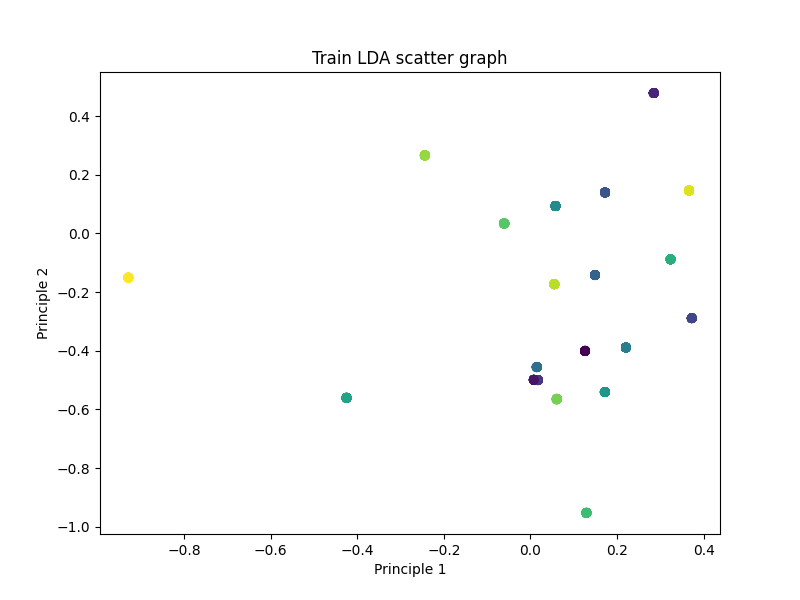
\includegraphics[width=0.7\textwidth]{Train LDA scatter graph.png}
		\caption{Train LDA scatter grap}
		\label{Train LDA scatter graph}
	\end{figure}

    \begin{figure}[H]
		\centering
		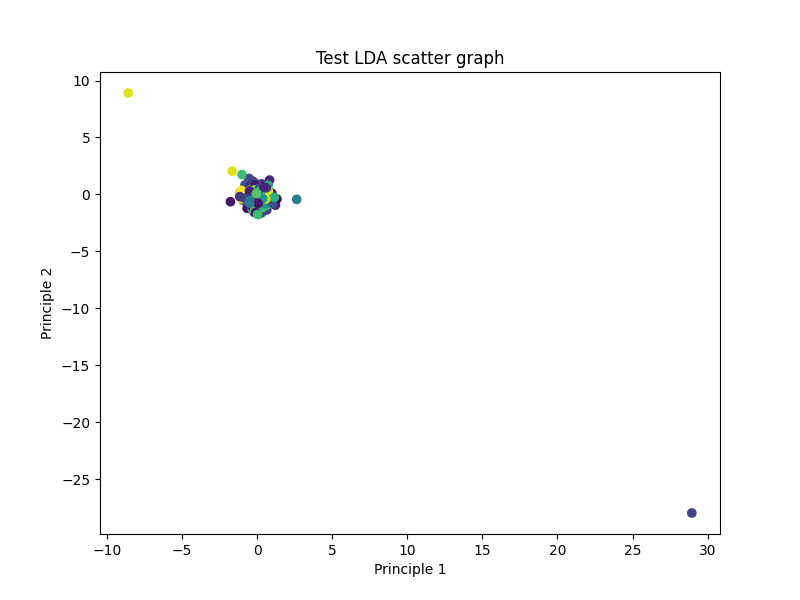
\includegraphics[width=0.7\textwidth]{Test LDA scatter graph.png}
		\caption{Test LDA scatter graph}
		\label{Test LDA scatter graph}
	\end{figure}
    我们把这个图放大一点看看:
    \begin{figure}[H]
		\centering
		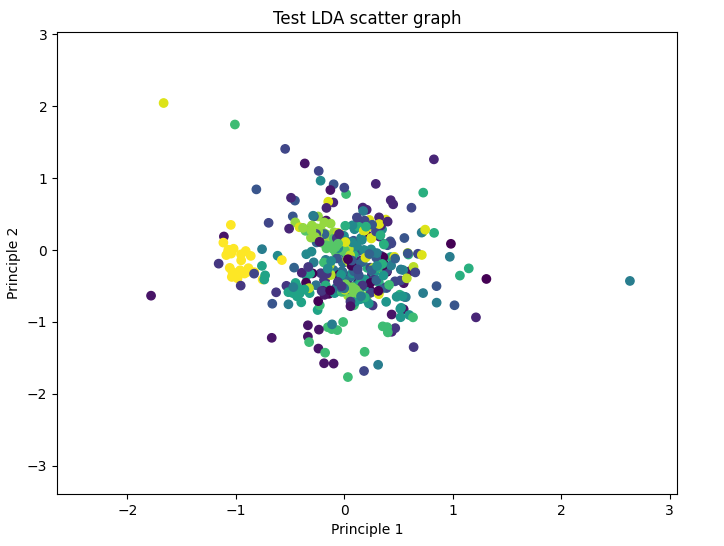
\includegraphics[width=0.7\textwidth]{bigger.png}
		\caption{Bigger Test LDA scatter graph}
		\label{Bigger Test LDA scatter graph}
	\end{figure}
    事实上,相比Sklearn的抽象降维,这个也至少把黄色分开了,sklearn的降维也是把黄色可以单独分开,所以其实效果还是可以。(我拿sklearn做了一个difftest)

    (3):截图如下:\\
    \begin{figure}[H]
		\centering
		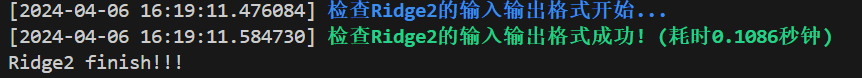
\includegraphics[width=0.7\textwidth]{Ridge2.png}
		\caption{Ridge2 test}
		\label{Ridge2 test}
	\end{figure}

    (4):截图如下:\\
    \begin{figure}[H]
		\centering
		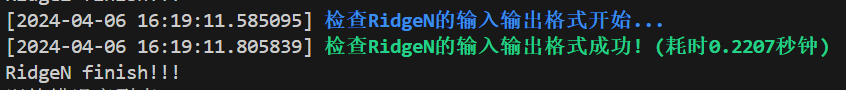
\includegraphics[width=0.7\textwidth]{RidgeN.png}
		\caption{RidgeN test}
		\label{RidgeN test}
	\end{figure}

    (5):截图如下:\\
    \begin{figure}[H]
		\centering
		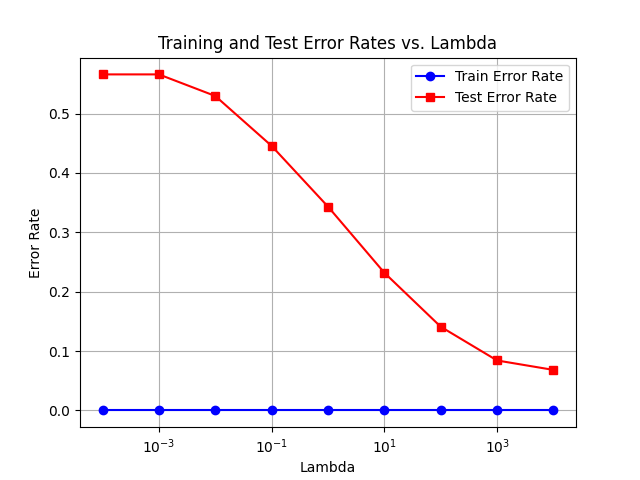
\includegraphics[width=0.7\textwidth]{HW2.png}
		\caption{HW2}
		\label{HW2}
	\end{figure}
    这个地方还是有一些疑惑的,为什么效果在训练集上能够达到100\%,虽然也不是不可能,但是有点离谱了

\end{solution}
\newpage

\section*{Acknowledgments}
允许与其他同样未完成作业的同学讨论作业的内容, 但需在此注明并加以致谢; 如在作业过程中, 参考了互联网上的资料或大语言模型的生成结果, 且对完成作业有帮助的, 亦需注明并致谢.\\

感谢人工智能学院221300012项远方同学对我的帮助,我们进行了友好的讨论,并得到了一个合理的结果。\\

感谢人工智能学院周志华老师课后关于决策树问题的深入浅出的讲解和分析!\\


\end{document}
